%
\documentclass[%
 reprint,
 amsmath,amssymb,
 aps,
]{revtex4-1}

\usepackage{graphicx}% Include figure files
\usepackage{dcolumn}% Align table columns on decimal point
\usepackage{bm}% bold math


\begin{document}


\title{Comparativa Datawarehouse vs DataLakes}
\author{Robles Flores, Anthony Richard	               (2016056192)}
\author{Estrella Palacios, Katherine Lizbeth			(2015050948)}
\author{Sosa Bedoya, Sharon Fiorela					(2016054460)}
\author{Torres Beltran , Johanna Andrea				(2020067849)}

		
\affiliation{%
 Universidad Privada de Tacna \textbackslash Facultad de Ingenieria \textbackslash Escuela Profesional de Ingenieria de Sistemas
}%

\begin{abstract}
\begin{center}
\textbf{Resumen}
\end{center}
Los almacenes de datos (data warehouses en inglés) toman cada día mayor importancia, a medida que las organizaciones pasan de esquemas de sólo recolección de datos a esquemas de análisis de los mismos. En este breve artículo se  tratará de brindar una explicación general de algunas metodologías, en este caso serán la metodología Kimball y la metodología Inmon.
\\

\begin{center}
\textbf{Abstract}
\end{center}
Data warehouses (data warehouses in English) are becoming increasingly important, as organizations move from data-only schemes to data analysis schemes. In this short article we will try to provide a general explanation of some methodologies, in this case they will be the Kimball methodology and the Inmon methodology.
\\
\end{abstract}



\maketitle

%\tableofcontents

\section {Introducción}\label{sec:1}

Actualmente las organizaciones utilizan la información y el conocimiento para apoyar la toma de sus decisiones estratégicas, y de este modo lograr sus metas y mejorar sus procesos.
Uno de los desafíos que enfrentan hoy las organizaciones, es el aumento de datos, lo que ha generado dos grandes problemas; el primero, identificar los datos relevantes para dar seguimiento a su estrategia organizacional, y lograr que se cumplan los planes con las metas establecidas.
 Y el segundo problema, la capacidad para administrar esta gran cantidad de datos.
Un almacén de datos  según Inmon, es una colección de datos orientada a un determinado ámbito (empresa, organización, etc.), integrado, no volatil y variable en el tiempo, que ayuda a la toma de decisiones en la entidad en la que se utiliza. 
Se trata, sobre todo, de un historial completo de la organización, mas alla de la informacion transaccional y operacional, almacenado en una base de datos diseñada para favorecer el análisis y la divulgación eficiente de datos (especialmente con herramientas OLAP, de procesamiento analítico en línea). Por otra parte Kimball la define como una copia de los datos transaccionales estructurados específicamente para consultas y análisis. 
En este breve artículo intentaremos brindar una explicación general de dos de las metodologías más usadas, la metodología de Kimball y metodología Inmon. \cite{estrella1}
%-----------------------------------------------------------------
\section{Objetivos}\label{sec:2}
\subsection{General:}
Dar una visión clara de BI, desde las perspectivas de los autores que sentaron las bases que son Ralph Kimball y Bill Inmon, para la mejora de las estrategias del negocio al que se desee implementar las herramientas de BI.
\subsection{Específicos:}
 Describir las metodologías propuestas por los principales autores de BI desde las perspectivas de sus creadores Ralph Kimball y Bill Inmon.


%-----------------------------------------------------------------
\section {Marco Teórico}

\subsection{DATAWAREHOUSE}	
Un almacén de datos (data warehouse, DW) /******************************************/

Consta de las siguientes características:
\begin{itemize}
		\item \textbf{Orientado a temas:} Los datos en la base de datos están organizados de manera que todos los elementos de datos relativos al mismo evento u objeto del mundo real queden unidos entre sí.	

\end{itemize}




%-------------------------------------------------

\subsection{DATAWAREHOUSE *************}
\begin{itemize}
	\item Descomposición funcional
	\item Diagrama de contexto
	\item Diagrama de flujo de datos
	\item Diagrama de transición de estados
	\item Pseudocódigo
\end{itemize}

	c. Modelo de datos. Se trabaja con 2 tipos de modelos:
		\begin{itemize}
			\item El Modelo de datos nos muestra los datos primitivos, tomando en cuenta el elemento tiempo, se plasman los cálculos que se realicen y finalmente se muestran sus relaciones.
		\end{itemize}

El Modelo de Datos del Data Warehouse. Los modelos anteriores nos deberán entregar la definición de los sujetos a los que estará orientado el Data Warehouse. Debe venir en 3 perspectivas y son explicadas en la siguiente tabla:


	d. Una vez que se tiene conocimiento de este modelo se deben tomar ciertas decisiones sobre el diseño del Data Warehouse. Entre estas decisiones tenemos las siguientes:
		\begin{itemize}
			\item Normalización, debemos decidir el grado al que nuestro Data Warehouse
			\item Granularidad
			\item Particiones
			\item  Minería de Datos
		\end{itemize}

	

%-------------------------------------------------
\subsection{DATAWAREHOUSE}
\begin{figure}[htb]
				\begin{center}
					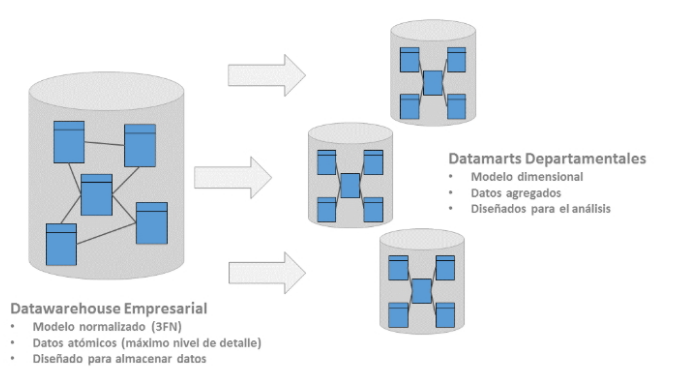
\includegraphics[width=9cm]{./IMAGENES/1}
				\end{center}
			\end{figure}

La arquitectura que plantea Bill Inmon consta de las siguientes partes: \cite{robles1}



\subsection{La estructura del DataWarehouse}	
En cuanto a la estructura interna del DataWarehouse, para Inmon la prioridad es que el modelo de datos esté construido en tercera 
/*******************************************************/

%-------------------------------------------------
\subsection{DATALAKES}	
La metodología se basa en lo que Kimball denomina Ciclo de Vida Dimensional del Negocio. Este ciclo de vida del proyecto de DW, está basado en cuatro principios básicos: 

\begin{itemize}
	\item Centrarse en el negocio: Hay que concentrarse en la identificación de los requerimientos del negocio y su valor asociado, y usar estos esfuerzos para desarrollar relaciones sólidas con el negocio, agudizando el análisis del mismo y la competencia consultiva de los implementadores. 
	\item Construir una infraestructura de información adecuada: Diseñaruna base de información única, integrada, fácil de usar, de alto rendimiento donde se reflejará la amplia gama de requerimientos de negocio identificados en la empresa. 
	\item Realizar entregas en incrementos significativos: crear el almacén de datos (DW) en incrementos entregables en plazos de 6 a 12 meses.
	\item Ofrecer la solución completa: proporcionar todos los elementos necesarios para entregar valor a los usuarios de negocios. 
\end{itemize}



%-------------------------------------------------
\subsection{IMPLEMENTACIONES DE DATALAKES}

/***********************************/
%-------------------------------------------------
\subsection{DATALAKES *********}

Ralph Kimball, plantea la idea de un enfoque dimensional para el diseño de un DW, y afirma que la unión de todos los DM de una organización constituye el DW corporativo, a lo cual se le conoce como el enfoque bottom-up.\\

 

%-------------------------------------------------

\subsection{COMPARACION DE DATAWAREHOUSE Y DATALAKES}	
xxxxxxxxxxxxxxxxxxxxxxxxxxxxxxxxxxxxxx

%-----------------------------------------------------------------
\section{Análisis}

\begin{itemize}
\item xxxxxxxxxxxxxxxxxxxxxxxxxxxxxxxxxxxxxx 
\item xxxxxxxxxxxxxxxxxxxxxxxxxxxxxxxxxxxxxx 
\end{itemize}
%-----------------------------------------------------------------
\section{Conclusiones}

\begin{itemize}
\item xxxxxxxxxxxxxxxxxxxxxxxxxxxxxxxxxxxxxx 
\item xxxxxxxxxxxxxxxxxxxxxxxxxxxxxxxxxxxxxx 

\end{itemize}


% Bibliografia.
%-----------------------------------------------------------------

\bibliographystyle{apalike}

\bibliography{Bibliografia}

\end{document}
